%%%%%%%%%%%%%%%%%%%%%%%%%%%%%%%%%%%%%%%%%
% Stylish Article
% LaTeX Template
% Version 2.1 (1/10/15)
%
% This template has been downloaded from:
% http://www.LaTeXTemplates.com
%
% Original author:
% Mathias Legrand (legrand.mathias@gmail.com) 
% With extensive modifications by:
% Vel (vel@latextemplates.com)
% Final ACS by:
% Juan Barbosa
% License:
% CC BY-NC-SA 3.0 (http://creativecommons.org/licenses/by-nc-sa/3.0/)
%
%%%%%%%%%%%%%%%%%%%%%%%%%%%%%%%%%%%%%%%%%
\documentclass[fleqn,10pt]{SelfArx}
%\usepackage[superscript]{cite}
\usepackage{wrapfig}
%----------------------------------------------------------------------------------------
%	ARTICLE INFORMATION
%----------------------------------------------------------------------------------------

\JournalInfo{Laboratorio Avanzado, No. 2, 04/07/2017} % Journal information
\Archive{ }

\PaperTitle{S\'intesis inorg\'anicas} %
%\Keywords{Keyword1 --- Keyword2 --- Keyword3} % Keywords - if you don't want any simply remove all the text between the curly brackets
%\newcommand{\keywordname}{Keywords} % Defines the keywords heading name

%----------------------------------------------------------------------------------------
%	ABSTRACT
%----------------------------------------------------------------------------------------

\Abstract{
%\begin{wrapfigure}{r}{0.45\textwidth}
%\centering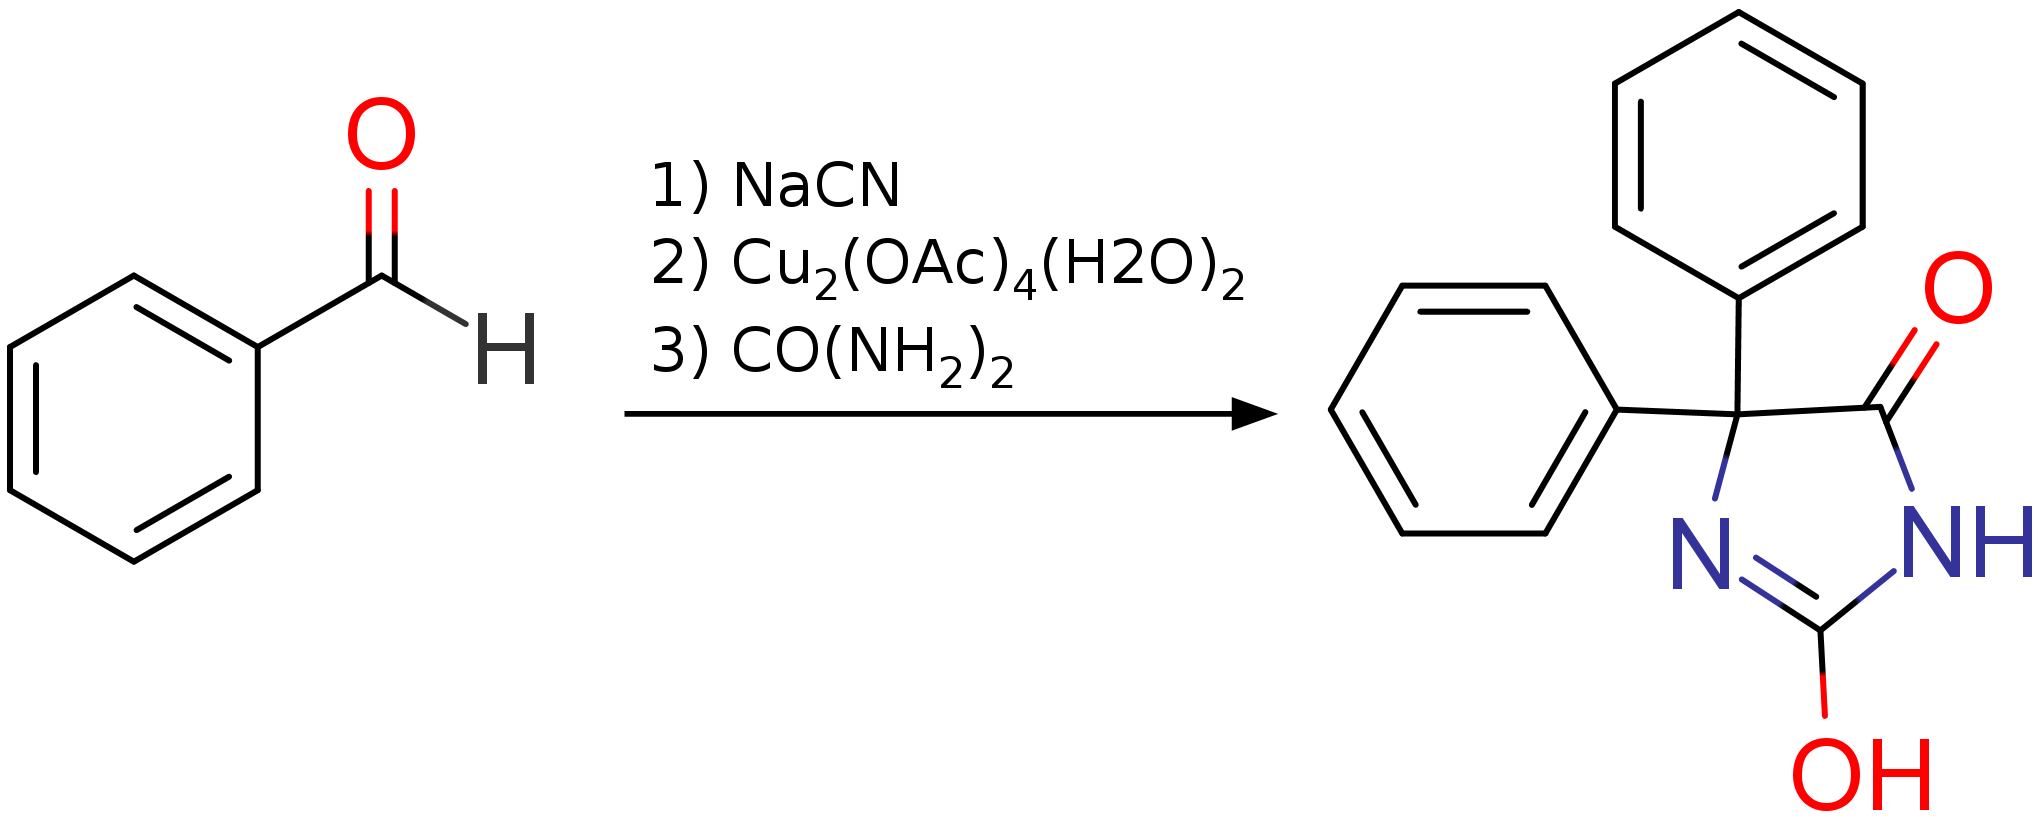
\includegraphics[scale=1]{structures/overall.png}
%\end{wrapfigure}
}

%----------------------------------------------------------------------------------------

\begin{document}

\flushbottom % Makes all text pages the same height

\maketitle % Print the title and abstract box

%\tableofcontents % Print the contents section

\thispagestyle{empty} % Removes page numbering from the first page



%----------------------------------------------------------------------------------------
%	ARTICLE CONTENTS
%----------------------------------------------------------------------------------------

\section*{Introducci\'on} % The \section*{} command stops section numbering

%------------------------------------------------

\section{Resultados y Discusi\'on}

\section{Conclusiones}

\section{Secci\'on experimental}
\subsection{S\'intesis de \ce{[Cu(NCS)(py)2(PPh3)]}}
La preparaci\'on de las sales se realiza usando dos soluciones 0.25 M (1.0 eq) de tiocianato de potasio y sulfato de cobre anhidro. Sobre un bal\'on con 25 mL de la soluci\'on de sulfato de cobre son adicionados 25 mL de la soluci\'on de tiocianato por goteo. La reacci\'on se calienta y agita por media hora, posteriormente se filtra el producto al vac\'io. Una mezcla con 0.2526 g ( eq) de tiocianato de cobre (I) y 0.5300 g ( eq) de trifenilfosfina se disuelve en 10 mL de piridina. La reacci\'on se lleva a cabo en reflujo por 3 horas.

\subsection{Reducci\'on con nanopart\'iculas}
Una soluci\'on tetrahidroborato de sodio (\ce{NaBH4}) se prepara con la disoluci\'on de 0.080 g del mismo en 10 mL de agua. Se prepara una segunda soluci\'on con 0.259 g de polivinilpirrolidina junto con 0.100 g de cloruro de cobalto hexahidratado en 10 mL de agua. La soluci\'on de \ce{NaBH4} se adiciona por goteo en presencia de ultrasonido. El producto obtenido se separa en dos mitades, una de las cuales se hace reaccionar con 0.1504 g de \textit{p}-nitrobenzaldehido y 0.2 mL de hidracina hidratada. La reacci\'on se sigue por cromatograf\'ia de placa delgada, usando diclorometano. El producto se obtiene por evaporaci\'on a presi\'on reducida luego de 90 minutos del inicio de la reacci\'on.

\subsection{S\'intesis de un cluster termocr\'omico}
Tres soluciones acuosas con vol\'umenes 15 mL, 30 mL y 10 mL son preparadas. La primera contiene 1.6205 g de sulfato de cobre pentahidratado, la segunda 0.5000 g de sulfito de sodio y la tercera 1.0800 g de yoduro de potasio. Sobre la segunda soluci\'on se adiciona \'acido sulf\'urico concentrado y se mezcla con la primera. Una vez disueltos los s\'olidos se adiciona la \'ultima soluci\'on a la mezcla. El yoduro de cobre obtenido se agrega a una soluci\'on 0.52 mL de piridina y 5 mL de acetonitrilo, sobre la misma se adicionan 0.7726 g de yoduro de potasio y 0.0332 g de \'acido asc\'orbico. La soluci\'on se agita por 15 minutos, posterior a los cuales se adicionan 25 mL de agua. El producto se filtra al vac\'io.  

%----------------------------------------------------------------------------------------
%	REFERENCE LIST
%----------------------------------------------------------------------------------------
\phantomsection
\bibliography{informe}
\bibliographystyle{unsrt}

%----------------------------------------------------------------------------------------
\newpage
\onecolumn
\section{Informaci\'on suplementaria}\label{sec: complementaria}

\end{document}